\newpage
\section{Basic Assembly Test}
In order to foster the development of the league and expand towards more complicated domains, an assembly challenge will be held. The focus is to show new and challenging aspects of assembly which can be performed by small service robots.

\subsection{Purpose and Focus of the Test}
The purpose of the \iaterm{Basic Assembly Test}{BAT} is to demonstrate basic assembly capabilities by the robots, like combining objects, by fitting or attaching them together.
The focus is on the manipulation towards assembly, e.g. force fitting or the preparation of objects to be attached by e.g. external devices and machines. This can include holding an object in place for another robot, machine or human to assemble it.

\subsection{Scenario Environment}
The arena used for this test contains all elements as for the Basic Navigation Test. In addition to environmental elements (such as walls, service areas, floor markers, etc.), different manipulatable objects will be placed on the service areas. On top of the service area, a car model will be mounted and fixed, so that the robot will not be able to move the car (see Fig \ref{fig:BAT_car}). The axle will be red, the tire blue and the car model will be neither.

\begin{figure} [h!]
\centering
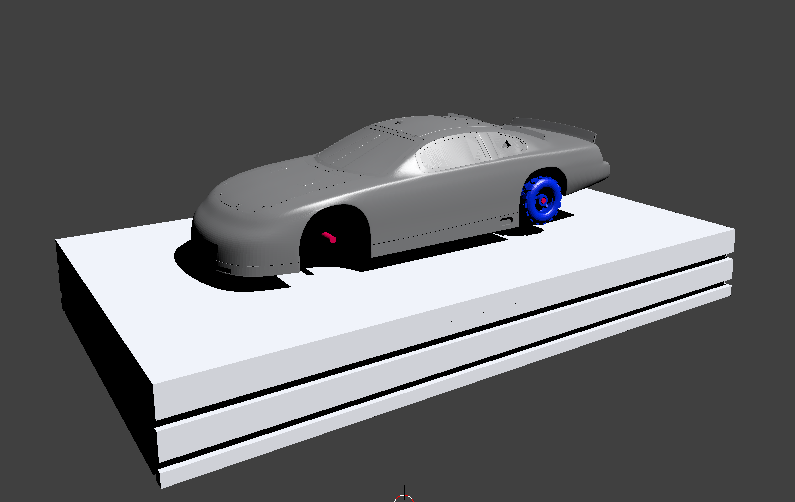
\includegraphics[width=0.8\textwidth ]{./images/BAT.png}
\caption{A example scene for the Basic Assembly Test. The actual car model may differ, but the wheels (\emph{blue}) need to be fitted onto the axes (\emph{red}).}
\label{fig:BAT_car}
\end{figure}


\subsection{Manipulation Objects}
The manipulation objects in this test may include the objects specified in Table, as they can still be inside of the arena and function as decoy objects. \ref{tab:manipulation_objects}.
The set of objects is extended by:

\begin{table}[p]
\begin{tabular}{|c|c|c|p{5cm}|}
\hline 
 & Symbolic Description & Mass & Details \\ 
\hline 
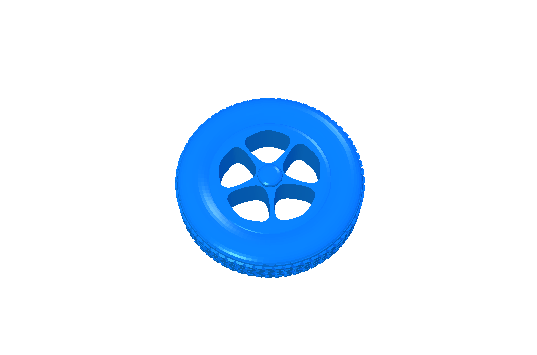
\includegraphics[width=3cm]{./images/BAT_Tire.png}  & T50 & 20 g & Radius: 50mm \newline
 Height: 34mm \\
\hline 
\end{tabular} 

\label{tab:bat_objects}
\caption{Examples of assembly objects}
\end{table}

All objects can be printed using a 3D-printer (e.g. axis and wheel), the car model is only for visualization purposes. All parts are available as STL files in the official \RCAW \emph{model} repository (see Section \ref{ssec:LeagueInfrastructure}).


\subsection{Task}
A single robot is used. The task consists of a sequence of assembly operations, with a small base movement in between. The objective is to collect a set of objects and perform an assembly option. The robot will be given instruction where to pick up the wheels and where to assemble them. The task is to fit the wheels onto the axes. The wheels and the axes need to be detected by the robot. A few wheels may be already assembled. Therefore it is necessary to detect where a wheel is still missing. The wheels designated for assembly will lie flat on the service areas.

\par
The task specification consists of: 
\begin{itemize}
	\item Location(s) of the wheels
	\item Location(s) where the assembly takes places
\end{itemize}

\subsection{Rules}
The following rules have to be obeyed:

\begin{itemize}
\item The order in which the teams have to perform will be determined by a draw.
\item At the beginning of a team's period, the team will get the task specification. 
\item The team must set-up the robot in the designated start area.
\item An assembly object counts as successfully assembled when it is attached to the correct object or is in place for the external device to perform the assembly.
\item An assembly objects counts as assembled wrong when it is assembled wrong (e.g. fitting a second tire on one axle)
\item The maximum time and the number of assemblies to be performed will be determined during the event by the TC.
\end{itemize}


\subsection{Scoring}
Points are awarded as follows:

\begin{itemize}
\item correct assembly:  \hfill 100 points
\item wrong assembly:  \hfill -100 points
\end{itemize}


